
\documentclass{standalone}
\usepackage[svgnames]{xcolor}
\usepackage{pgfplots}
\pgfplotsset{compat=newest}
\usepackage[sfdefault]{FiraSans}
\usepackage{FiraMono}
\renewcommand*\familydefault{\sfdefault}
\begin{document}
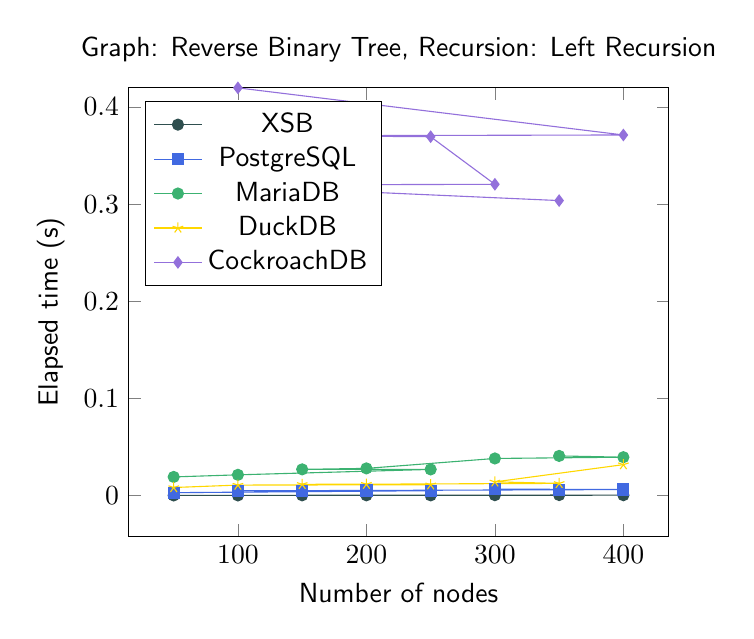
\begin{tikzpicture}
    \begin{axis}[
        title={Graph: Reverse Binary Tree, Recursion: Left Recursion},
        xlabel={Number of nodes},
        ylabel={Elapsed time (s)},
        legend pos={north west},
        ymax=0.41976059599983273
    ]
    \addplot+[DarkSlateGray, mark options={color=DarkSlateGray}] coordinates {(50,3.99351119995117e-05) (100,7.343292236328125e-05) (250,0.00013792514801025401) (150,0.00017452239990234348) (200,0.000176548957824707) (400,0.000298619270324707) (300,0.00034201145172119097) (350,0.000445842742919922)};
\addlegendentry{XSB}
\addplot+[RoyalBlue, mark options={color=RoyalBlue}] coordinates {(50,0.002875510999842845) (250,0.00493507049998243) (100,0.004962819500065052) (150,0.005002099500075019) (200,0.005150974000002861) (350,0.005861655499984408) (400,0.006087229000058869) (300,0.00655161399993176)};
\addlegendentry{PostgreSQL}
\addplot+[MediumSeaGreen, mark options={color=MediumSeaGreen}] coordinates {(50,0.019101973500255554) (100,0.021253678999983094) (250,0.026833034999981464) (150,0.02688620300000366) (200,0.027886849499964228) (300,0.038113121000151295) (400,0.0394251620000432) (350,0.040728427499971076)};
\addlegendentry{MariaDB}
\addplot+[Gold, mark options={color=Gold}] coordinates {(50,0.008202444000062314) (100,0.010704105000058917) (250,0.011032004499838877) (150,0.011473908999960258) (200,0.01160856750016137) (350,0.01245864900010929) (300,0.014004304000081902) (400,0.03174599250019128)};
\addlegendentry{DuckDB}
\addplot+[MediumPurple, mark options={color=MediumPurple}] coordinates {(350,0.30369652599983965) (200,0.312483537999924) (50,0.31960767349983144) (300,0.32043739199980337) (250,0.3694382214998768) (150,0.37045632250010385) (400,0.37125362500000847) (100,0.41976059599983273)};
\addlegendentry{CockroachDB}

    \end{axis}
\end{tikzpicture}
\end{document}
